\documentclass[12pt,a4paper]{ctexart}  
\usepackage[utf8]{inputenc}
\usepackage{easyReview}
\usepackage[T1]{fontenc}
\usepackage{amsmath}
\usepackage{fancyhdr}  %设置论文的页眉页脚
\usepackage{amsfonts}
\usepackage{multirow}
\usepackage{booktabs}
\usepackage{amssymb}
\usepackage{amsmath}
\usepackage{multirow}   %???
\usepackage{booktabs}
\usepackage{subcaption}
\usepackage{float}
\usepackage{amsfonts}
\usepackage{mathrsfs}
\usepackage{amssymb}
\usepackage{mathrsfs}
\usepackage{bm}
\usepackage{extarrows}  %等号上面加文字
\usepackage{extarrows}
\usepackage{wasysym}   %添加表情
\usepackage{graphbox}  %图片放右侧
\usepackage{graphicx}
%\usepackage{subfig}
%\usepackage{subfloat}
\usepackage[colorlinks,linkcolor=red,anchorcolor=blue,citecolor=green]{hyperref}
\usepackage{amssymb}
\usepackage{mathrsfs}
\usepackage{cases}   %多个公式一起编号
\usepackage{color}
\usepackage{tcolorbox}
\usepackage{listings}
\usepackage{xcolor}
\usepackage[framemethod=tikz]{mdframed}  %高亮显示某段文字
\usepackage[left=2.00cm, right=2.00cm, top=2.00cm, bottom=2.00cm]{geometry}

\newcommand{\RNum}[1]{\uppercase\expandafter{\romannumeral #1\relax}}        %添加罗马数字
\newtheorem{theorem}{定理}[section] % 定义一个定理环境，名为定理，编号依赖于 section
\newtheorem{lemma}[theorem]{Lemma} % 定义一个引理环境，名为引理，编号与定理共用
\newtheorem{definition}[theorem]{定义}
\newtheorem{example}[theorem]{例}
\newtheorem{exercise}[theorem]{\textcolor{blue} {练习}}
\newtheorem{problem}[theorem]{问题}
\newtheorem{property}[theorem]{性质}
\newtheorem{proposition}[theorem]{命题}
\newtheorem{remark}[theorem]{Remark}
\newtheorem{algorithm}[theorem]{算法}
\pagestyle{fancy}  %定义页码，页眉，页脚
\cfoot{\thepage}  %去掉页脚中间部分
\lhead{{《最优化理论与方法》实验报告}}


\begin{document}


% 我们开始自定义封面，首先设置封面不显示页号
% \pagestyle{empty}
% 来一个无法拒绝的垂直间距，大约是 12 个 M 字符的长度
\vspace*{6em}

\begin{figure}[H]
	\centering
	
\includegraphics[width=0.4\linewidth]{picture/HNUlogo}
\end{figure}
\vspace*{4em}
% 标题
\begin{center}
{\Huge \bf 《最优化算法与理论》 实验报告}  %\bigskip  % 垂直间距
\end{center}
\vspace{4em}  % 垂直间距
% 信息
\begin{center}
{\Large  % 这里的字号也可以用别的方式修改

{\bf\makebox[4em][s]{实验序号}}: \underline{\makebox[13em][l]{~~~~~~~~~~~~}}\\
{\bf\makebox[4em][s]{实验内容}}: \underline{\makebox[13em][l]{~~~~~~~~~~~~}}\\
{\bf\makebox[4em][s]{班~~~~级}}: \underline{\makebox[13em][l]{~~~~~~~~~~~~}}\\
{\bf\makebox[4em][s]{学~~~~号}}: \underline{\makebox[13em][l]{~~~~~~~~~~~~}}\\
{\bf\makebox[4em][s]{姓~~~~名}}: \underline{\makebox[13em][l]{~~~~~~~~~~~~}}\\
{\bf\makebox[4em][s]{完成日期}}: \underline{\makebox[13em][l]{~~~~~~~~~~~~年~~~~~~月~~~~~~日~~~~}}\\

}
\end{center}
\clearpage

\newpage

\tableofcontents
\newpage

\section{实验内容之一: 黄金分割法}
\subsection{黄金分割法程序设计及运行结果}
我们用 C 语言编写程序实现了黄金分割法{\color {blue} （程序见作业附件压缩文件包）}. 我们应用程序
计算作业练习 1 中问题, 运行结果截图如下：
\begin{figure}[H]
	\centering
	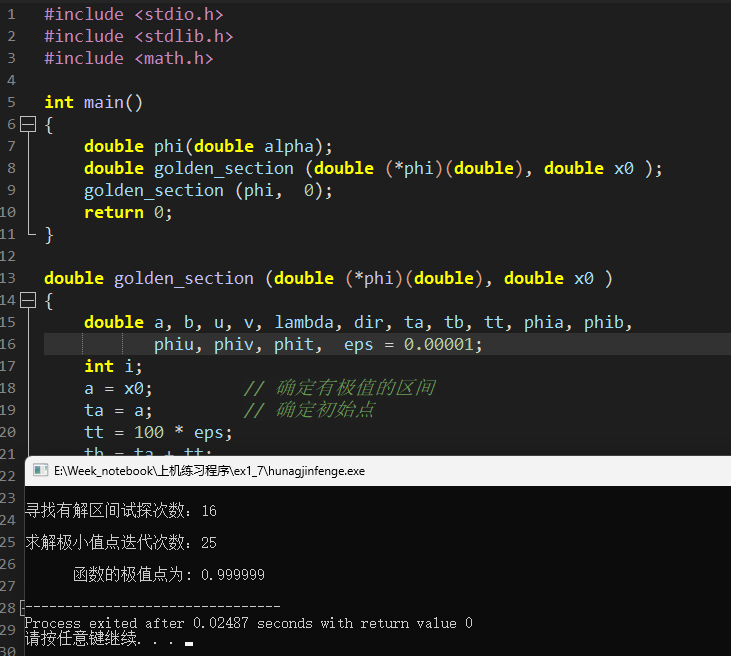
\includegraphics[width=0.9\linewidth]{picture/1}
	\caption{黄金分割法程序运行界面截图.}
	\label{fig:2}
\end{figure}
\subsection{程序运行情况说明及实验心得}
\begin{itemize}
  \item [](1) 寻找有解区间时的试探区间长度的选择对程序的效率影响较大;
  \item [](2) 算法还需要完善, 使之能有效求解病态问题的极小值点;
  \item [](3) 可将一元函数的插值法用于提升程序运算效率;
\end{itemize}


\section{实验内容之二:**** }
\subsection{****序设计及运行结果}
......
\subsection{程序运行情况说明及实验心得}
......

\section{实验内容之三:**** }
\subsection{****序设计及运行结果}
......
\subsection{程序运行情况说明及实验心得}
......


\end{document}


























